\documentclass{article}
\usepackage[margin=1in]{geometry}
\usepackage{amsmath,amsthm,amssymb,mathrsfs}
\usepackage{graphicx}
\usepackage[pdfencoding=auto, psdextra]{hyperref}
\usepackage[figurename=Figure]{caption}
% Consider adding natbib if you prefer author-year citations or need more control
% \usepackage[numbers]{natbib} % Use numbers for citations like the original
\usepackage{booktabs} % For better tables in the comparison section
\usepackage{enumitem} % For custom list labels if needed
\usepackage{tikz,tikz-cd}
\usetikzlibrary{positioning, arrows.meta}

\newtheorem{theorem}{Theorem}
\newtheorem{prop}{Proposition}
\newtheorem{remark}{Remark}
\newtheorem{conjecture}{Conjecture}
\newtheorem{definition}{Definition}

\newcommand{\mathpdf}[2]{\texorpdfstring{$#1$}{#2}}

\title{Sprecher Networks: A Trainable Architecture \\ Based on the Kolmogorov--Arnold--Sprecher Theorem}
\author{
  Christian Hägg\thanks{Department of Mathematics, Stockholm University, Stockholm, Sweden. Email: \texttt{hagg@math.su.se}} \and
  Kathlén Kohn\thanks{Department of Mathematics, KTH Royal Institute of Technology, Stockholm, Sweden. Email: \texttt{kathlen@kth.se}} \and
  Giovanni Luca Marchetti\thanks{Department of Mathematics, KTH Royal Institute of Technology, Stockholm, Sweden. Email: \texttt{glma@kth.se}} \and
  Boris Shapiro\thanks{Department of Mathematics, Stockholm University, Stockholm, Sweden. Email: \texttt{shapiro@math.su.se}}
}
\date{\today} % Using \today or leave empty

\begin{document}

\maketitle

\begin{abstract}
We present \emph{Sprecher Networks} (SNs), a family of trainable neural architectures inspired by the classical Kolmogorov--Arnold--Sprecher (KAS) construction for approximating multivariate continuous functions. Distinct from Multi-Layer Perceptrons (MLPs) with fixed node activations and Kolmogorov-Arnold Networks (KANs) featuring learnable edge activations, SNs utilize shared, learnable splines (\emph{monotonic} and \emph{general}) within structured blocks incorporating explicit learnable shifts and mixing weights. Our approach directly realizes Sprecher's specific 1965 ``sum of shifted splines'' formula in its single-layer variant and extends it to deeper, multi-layer compositions. We discuss theoretical motivations, implementation details, compare SNs with related architectures (MLPs, KANs, and networks with learnable node activations), and explore potential advantages in interpretability, universality, and parameter efficiency.
\end{abstract}

\section{Introduction and historical background}
Approximation of continuous functions by sums of univariate functions has been a recurring theme in mathematical analysis and neural networks. The Kolmogorov--Arnold Representation Theorem \cite{kolmogorov, arnold} established that any multivariate continuous function $f : [0,1]^d \to \mathbb{R}$ can be represented as a finite composition of continuous functions of a single variable and the addition operation. Specifically, Kolmogorov (1957) showed that such functions can be represented as a finite sum involving univariate functions applied to sums of other univariate functions of the inputs.

\vspace{1mm}
\textbf{David Sprecher's 1965 construction.} In his 1965 landmark paper \cite{sprecher1965}, David Sprecher provided a constructive proof and a specific formula realizing the Kolmogorov--Arnold representation. He showed that any continuous function $f:[0,1]^n \to \mathbb{R}$ could be represented as:
$$f(\mathbf{x})=\sum_{q=0}^{2n}\Phi\Bigl(\,\sum_{p=1}^{n}\lambda_p\,\phi\bigl(x_p+\eta\,q\bigr)+q\Bigr)$$
for a single \emph{monotonic} inner function $\phi$, a continuous outer function $\Phi$, a constant shift parameter $\eta > 0$, and constants $\lambda_p$. This construction simplified the representation by using only one inner function $\phi$, relying on shifts of the input coordinates ($x_p + \eta q$) and an outer summation index shift ($+q$) to achieve universality. The key insight of \emph{shifting input coordinates} and summing evaluations under inner and outer univariate maps is central to Sprecher's specific result.

\vspace{1mm}
\textbf{Modern context.} Recent work has revitalized interest in leveraging Kolmogorov-Arnold representations for modern deep learning. Notably, Kolmogorov-Arnold Networks (KANs) \cite{liu2024kan} were introduced, proposing an architecture with learnable activation functions (splines) placed on the \emph{edges} of the network graph, replacing traditional linear weights and fixed node activations.

\vspace{1mm}
\textbf{Architectural landscape.} Understanding how novel architectures relate to established ones is crucial. Standard Multi-Layer Perceptrons (MLPs) \cite{haykin1994neural} employ fixed nonlinear activation functions at nodes and learnable linear weights on edges, justified by the Universal Approximation Theorem \cite{cybenko1989approximation, hornik1989multilayer}. Extensions include networks with \emph{learnable activations on nodes}, sometimes called Adaptive-MLPs or Learnable Activation Networks (LANs) \cite{goyal2019learning, zhang2022neural, liu2024kan} (Appendix B), which retain linear edge weights but make the node non-linearity trainable. KANs \cite{liu2024kan} represent a more significant departure, moving learnable splines to edges and eliminating linear weights entirely, using simple summation at nodes. Sprecher Networks (SNs), as we detail below, propose a distinct approach derived directly from Sprecher's 1965 formula. SNs employ function blocks containing shared learnable splines ($\phi, \Phi$), learnable mixing weights ($\lambda$), and explicit structural shifts ($\eta, q$). This structure offers a different alternative within the landscape of function approximation networks.

\section{Motivation and overview of Sprecher Networks}
While MLPs are the workhorse of deep learning, architectures inspired by KAS representations offer potential benefits, particularly in interpretability and potentially parameter efficiency for certain function classes. KANs explore one direction by placing learnable functions on edges. Our \emph{Sprecher Networks} (SNs) explore a different direction, aiming to directly implement Sprecher's constructive formula within a trainable framework and extend it to deeper architectures.

SNs are built upon the following principles, directly reflecting Sprecher's formula:
\begin{itemize}
    \item Each functional block (mapping between layers) is organized around a shared \emph{monotonic} spline $\phi(\cdot)$ and a shared \emph{general} spline $\Phi(\cdot)$, both learnable.
    \item Each block incorporates a learnable scalar shift $\eta$ applied to inputs based on the output index $q$.
    \item Each block includes learnable mixing weights $\lambda_{i,q}$ that combine contributions from different input dimensions.
    \item The structure explicitly includes the additive shift $q$ inside the outer spline $\Phi$, mimicking Sprecher's formulation.
\end{itemize}
Our architecture generalizes this classical single-layer shift-and-sum construction to a multi-layer network by composing these functional units, which we term \emph{Sprecher blocks}. The mapping from one hidden layer representation to the next is realized by such a block. Unlike MLPs with fixed node activations, LANs with learnable node activations, or KANs with learnable edge activations, SNs concentrate their learnable non-linearity into the two shared splines per block, applied in a specific structure involving shifts and learnable linear weights. Diversity in the transformation arises from the mixing weights ($\lambda$) and the index-dependent shifts ($q$).

Concretely, each Sprecher block applies the transformation:
$$ (x_i)_{i=1}^{d_{\mathrm{in}}} \;\mapsto\; \Bigl[\Phi\Bigl(\sum_{i=1}^{d_{\mathrm{in}}}\lambda_{i,q}\,\phi(x_i+\eta\,q)+q\Bigr)\Bigr]_{q=0}^{d_{\mathrm{out}}-1}.$$
For scalar outputs, the outputs of the final Sprecher block are aggregated (via summation over $q$). For vector outputs, an additional block is typically (?) used without final summation.

In Sprecher's original work, one layer (block) with $d_{\mathrm{out}} = 2n+1$ outputs (where $n=d_{\mathrm{in}}$) was sufficient for universality. Our approach stacks $L$ Sprecher blocks to create a deep network progression:
$$ d_0 \to d_1 \to \cdots \to d_{L-1} \to d_L, $$
where $d_0=d_{\mathrm{in}}$ is the input dimension, and $d_L$ is the dimension of the final hidden representation before potential aggregation or final mapping. This multi-block composition provides a deeper analog of the KAS construction, aiming for potentially enhanced expressive power or efficiency for complex compositional functions. However, it's important to note that rigorous universality is established only for a single block with scalar output (directly from Sprecher's theorem); the universality of networks with \(L>1\) blocks or vector-valued outputs remains conjectural (see Section~\ref{sec:universality}).

\begin{definition}[Network notation]
Throughout this paper, we denote Sprecher Network architectures using arrow notation of the form $d_{\mathrm{in}}\to[d_1,d_2,\ldots,d_L]\to d_{\mathrm{out}}$, where $d_{\mathrm{in}}$ is the input dimension, $[d_1,d_2,\ldots,d_L]$ represents the hidden layer dimensions (widths), and $d_{\mathrm{out}}$ is the final output dimension of the network (after potential summation). For example, $2\to[5,3,8]\to1$ describes a network with 2-dimensional input, three hidden layers of widths 5, 3, and 8 respectively, and a scalar output (implying the final block's outputs of dimension 8 are summed). $2\to[5,3]\to4$ describes a network with 2-dimensional input, two hidden layers of widths 5 and 3, and a 4-dimensional vector output (implying an additional output block maps from dimension 3 to 4 without summation). When input or output dimensions are clear from context, we may use the abbreviated notation $[d_1,d_2,\ldots,d_L]$ to focus on the hidden layer structure.
\end{definition}

\section{Core architectural details}
In our architecture, the fundamental building unit is the \emph{Sprecher block}. The network is composed of a sequence of Sprecher blocks, each performing a shift-and-sum transformation inspired by Sprecher's original construction.

\subsection{Sprecher block structure}
A Sprecher block transforms an input vector $\mathbf{x} \in \mathbb{R}^{d_{\mathrm{in}}}$ to an output vector $\mathbf{h} \in \mathbb{R}^{d_{\mathrm{out}}}$. This transformation is implemented using the following shared, learnable components specific to that block:
\begin{itemize}
    \item \textbf{Monotonic spline $\phi(\cdot)$:} An increasing piecewise-linear function, typically defined on a fixed interval like $[0,1]$. This function is shared across all input-output connections within the block and its coefficients are learnable. (Strict?) Monotonicity is enforced during training (see Section \ref{sec:implementation}).
    \item \textbf{General spline $\Phi(\cdot)$:} A piecewise-linear function (without monotonicity constraints) defined on a potentially wider interval (e.g., $[-10, 20]$), which might be learnable or fixed depending on configuration. This function is also shared across the block and its coefficients are learnable.
    \item \textbf{Mixing weights matrix $\lambda$:} A matrix $\{\lambda_{i,q}\}$ of size $d_{\mathrm{in}} \times d_{\mathrm{out}}$, whose entries are learnable. These weights linearly combine the contributions from different input dimensions after transformation by $\phi$.
    \item \textbf{Shift parameter $\eta$:} A learnable scalar $\eta > 0$. This parameter controls the magnitude of the input shift $x_i + \eta q$, which depends on the output index $q$.
\end{itemize}

Concretely, given an input vector $\mathbf{x} = (x_1, \dots, x_{d_{\mathrm{in}}}) \in \mathbb{R}^{d_{\mathrm{in}}}$, a single Sprecher block (indexed implicitly by $\ell$, with parameters $\phi^{(\ell)}, \Phi^{(\ell)}, \eta^{(\ell)}, \lambda^{(\ell)}$) computes the $q$-th component of its output vector $\mathbf{h} \in \mathbb{R}^{d_{\mathrm{out}}}$ (where $q=0, \dots, d_{\mathrm{out}}-1$) via:
$$ h_q = \text{Block}_{\phi,\Phi,\eta,\lambda}(\mathbf{x})_q = \Phi^{(\ell)}\Biggl(\,\sum_{i=1}^{d_{\mathrm{in}}}\lambda^{(\ell)}_{i,q}\,\phi^{(\ell)}\Bigl(x_i+\eta^{(\ell)}\,q\Bigr) + q\Biggr). $$
Note the explicit inclusion of the outer shift $q$ inside the argument of $\Phi$, directly mirroring Sprecher's formula.

In a network with multiple layers, each Sprecher block (indexed by $\ell=1, \dots, L$ or $L+1$) uses its own independent set of shared parameters $(\phi^{(\ell)}, \Phi^{(\ell)}, \eta^{(\ell)}, \lambda^{(\ell)})$. The block operation implements a specific form of transformation: each input coordinate $x_i$ is first shifted by an amount depending on the output index $q$ and the shared shift parameter $\eta^{(\ell)}$, then passed through the shared monotonic spline $\phi^{(\ell)}$. The results are linearly combined using the learnable mixing weights $\lambda^{(\ell)}_{i,q}$, shifted again by the output index $q$, and finally passed through the shared general spline $\Phi^{(\ell)}$. Stacking these blocks creates a deep, compositional representation.

\subsection{Layer composition and final mapping}
Let $L$ be the number of hidden layers specified by the architecture $[d_1, \dots, d_L]$. In our framework, a "hidden layer" corresponds to the vector output of a Sprecher block. The mapping from the representation at layer $\ell-1$ to layer $\ell$ is implemented by the $\ell$-th Sprecher block.

Let the input to the network be $\mathbf{h}^{(0)} = \mathbf{x} \in \mathbb{R}^{d_0}$ (where $d_0 = d_{\mathrm{in}}$). The output of the $\ell$-th Sprecher block ($\ell = 1, \dots, L$) is the vector $\mathbf{h}^{(\ell)} \in \mathbb{R}^{d_\ell}$, computed component-wise as:
\begin{align}
    \label{eq:SN}\mathbf{h}^{(\ell)}_q = \Phi^{(\ell)}\Biggl(\,\sum_{i=1}^{d_{\ell-1}} \lambda^{(\ell)}_{i,q}\,\phi^{(\ell)}\Bigl(\mathbf{h}^{(\ell-1)}_i+\eta^{(\ell)}\,q\Bigr) + q\Biggr),\quad q=0,\dots,d_\ell-1.
\end{align}

The composition of these blocks and the final output generation depend on the desired final output dimension $m=d_{\mathrm{out}}$:

\paragraph{(a) Scalar output ($m=1$):}
The network consists of exactly $L$ Sprecher blocks. The output of the final block, $\mathbf{h}^{(L)} \in \mathbb{R}^{d_L}$, is aggregated by summation to yield the scalar output:
$$ f(\mathbf{x}) = \sum_{q=0}^{d_L-1} \mathbf{h}^{(L)}_q. $$
If we define the operator for the $\ell$-th block as $T^{(\ell)}: \mathbb{R}^{d_{\ell-1}} \to \mathbb{R}^{d_\ell}$, where
$$ \Bigl(T^{(\ell)}(z)\Bigr)_q = \Phi^{(\ell)}\Biggl(\,\sum_{i=1}^{d_{\ell-1}} \lambda^{(\ell)}_{i,q}\,\phi^{(\ell)}\Bigl(z_i+\eta^{(\ell)}\,q\Bigr) + q\Biggr), $$
then the overall function is
$$ f(\mathbf{x}) = \sum_{q=0}^{d_L-1} \Bigl(T^{(L)} \circ T^{(L-1)} \circ \cdots \circ T^{(1)}\Bigr)(\mathbf{x})_q. $$
This network uses $L$ blocks and $2L$ shared spline functions in total (one pair $(\phi^{(\ell)}, \Phi^{(\ell)})$ per block).

\paragraph{(b) Vector-valued output ($m>1$):}
When the target function $f$ maps to $\mathbb{R}^m$ with $m>1$, the network first constructs the $L$ hidden layers as above, yielding a final hidden representation $\mathbf{h}^{(L)} \in \mathbb{R}^{d_L}$. An \emph{additional} output block (block $L+1$) is then appended to map this representation $\mathbf{h}^{(L)}$ to the final output space $\mathbb{R}^m$. This $(L+1)$-th block operates \emph{without} a final summation over its output index. It computes the final output vector $\mathbf{y} \in \mathbb{R}^m$ as:
$$ y_q = \Bigl(T^{(L+1)}(\mathbf{h}^{(L)})\Bigr)_q = \Phi^{(L+1)}\Biggl(\,\sum_{r=0}^{d_L-1} \lambda^{(L+1)}_{r,q}\,\phi^{(L+1)}\Bigl(\mathbf{h}^{(L)}_r+\eta^{(L+1)}\,q\Bigr)+q\Biggr), $$
for $q=0,\dots,m-1$. The network output function is then:
\begin{equation}\label{eq:defsn}
f(\mathbf{x}) = \mathbf{y} = \Bigl(T^{(L+1)} \circ T^{(L)} \circ \cdots \circ T^{(1)}\Bigr)(\mathbf{x}) \in \mathbb{R}^m. 
\end{equation}
In this configuration, the network uses $L+1$ blocks and involves $2(L+1)$ shared spline functions. The extra block serves as a trainable output mapping layer, transforming the final hidden representation $\mathbf{h}^{(L)}$ into the desired $m$-dimensional output vector.

\medskip
In summary: for $L \ge 1$ hidden layers, a scalar-output SN uses $L$ blocks and $2L$ shared splines. A vector-output SN (with $m>1$) uses $L+1$ blocks and $2(L+1)$ shared splines. This structure provides a natural extension of Sprecher's original scalar formula to the vector-valued setting.

% Perhaps the illustration below is a bit too repetitive?
\medskip
We illustrate the vector-output case ($m>1$) for a network architecture $d_0\to[d_1,d_2,d_3]\to m$ (i.e., $L=3$ hidden layers). Let $X^{(0)}$ be the input $\mathbf{x}$.
\begin{center}
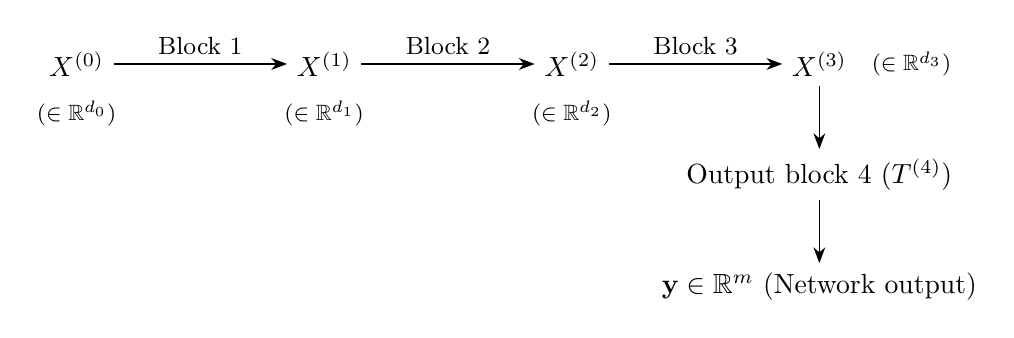
\begin{tikzpicture}[
    node distance=0.8cm and 2.2cm, % Vertical and horizontal node distances
    block/.style={font=\small}, % Style for block labels
    dim/.style={font=\footnotesize} % Style for dimension labels
  ]
    % Define nodes
    \node (X0)                                      {$X^{(0)}$};
    \node (L0) [below=0.07cm of X0, dim]             {$(\in \mathbb{R}^{d_0})$};
    \node (X1) [right=of X0]                        {$X^{(1)}$};
    \node (L1) [below=0.07cm of X1, dim]             {$(\in \mathbb{R}^{d_1})$};
    \node (X2) [right=of X1]                        {$X^{(2)}$};
    \node (L2) [below=0.07cm of X2, dim]             {$(\in \mathbb{R}^{d_2})$};
    \node (X3) [right=of X2]                        {$X^{(3)}$};
    \node (L3) [right=0.07cm of X3, dim]             {$(\in \mathbb{R}^{d_3})$};
    \node (OB) [below=of X3]                        {Output block 4 $(T^{(4)})$};
    \node (Y)  [below=of OB]                        {$\mathbf{y} \in \mathbb{R}^m$ (Network output)};

    % Draw arrows
    \draw[-{Stealth[length=2mm]}] (X0) -- node[above, block] {Block 1} (X1);
    \draw[-{Stealth[length=2mm]}] (X1) -- node[above, block] {Block 2} (X2);
    \draw[-{Stealth[length=2mm]}] (X2) -- node[above, block] {Block 3} (X3);
    \draw[-{Stealth[length=2mm]}] (X3) -- (OB); % Vertical arrow
    \draw[-{Stealth[length=2mm]}] (OB) -- (Y);  % Vertical arrow
\end{tikzpicture}
\end{center}
Here, $X^{(\ell)} = \mathbf{h}^{(\ell)}$ denotes the output vector of the $\ell$-th Sprecher block. Each block $T^{(\ell)}$ internally uses its own pair of shared splines $(\phi^{(\ell)}, \Phi^{(\ell)})$, mixing weights $\lambda^{(\ell)}$, and shift $\eta^{(\ell)}$. The final output block $T^{(4)}$ maps the representation $X^{(3)}$ to the final $m$-dimensional output $\mathbf{y}$ without subsequent summation.

\subsection{Illustrative expansions (scalar output)}
To further clarify the compositional structure for the scalar output case ($m=1$), we write out the full expansions for networks with $L=1, 2, 3$ hidden layers.

\subsubsection{Single hidden layer ($L=1$)}
For a network with architecture $d_{\mathrm{in}}\to[d_1]\to1$ (i.e., $d_0=d_{\mathrm{in}}$), the network computes:
$$f(\mathbf{x}) = \sum_{q=0}^{d_1-1} \mathbf{h}^{(1)}_q = \sum_{q=0}^{d_1-1} \Phi^{(1)}\Biggl(\sum_{i=1}^{d_0} \lambda^{(1)}_{i,q}\,\phi^{(1)}\Bigl(x_i+\eta^{(1)}\,q\Bigr)+q\Biggr).$$
This precisely reproduces Sprecher's 1965 construction if we choose $d_1=2d_0+1$ and identify $\phi^{(1)}=\phi$, $\Phi^{(1)}=\Phi$, and $\lambda^{(1)}_{i,q} = \lambda_i$ (independent of $q$).

\subsubsection{Two hidden layers ($L=2$)}
Let the architecture be $d_0\to[d_1, d_2]\to1$. The intermediate output $\mathbf{h}^{(1)} \in \mathbb{R}^{d_1}$ is computed as:
$$\mathbf{h}^{(1)}_r=\Phi^{(1)}\Bigl(\sum_{i=1}^{d_0}\lambda^{(1)}_{i,r}\,\phi^{(1)}\Bigl(x_i+\eta^{(1)}\,r\Bigr)+r\Bigr),\quad r=0,\dots,d_1-1.$$
The second block computes $\mathbf{h}^{(2)} \in \mathbb{R}^{d_2}$ using $\mathbf{h}^{(1)}$ as input:
$$\mathbf{h}^{(2)}_q=\Phi^{(2)}\Bigl(\sum_{r=0}^{d_1-1}\lambda^{(2)}_{r,q}\,\phi^{(2)}\Bigl(\mathbf{h}^{(1)}_r+\eta^{(2)}\,q\Bigr)+q\Bigr),\quad q=0,\dots,d_2-1.$$
The final network output is the sum over the components of $\mathbf{h}^{(2)}$: $f(\mathbf{x})=\sum_{q=0}^{d_2-1}\mathbf{h}^{(2)}_q$. Substituting $\mathbf{h}^{(1)}$, the fully expanded form is:
\begin{equation}\label{eq:two-layer-restored}
f(\mathbf{x})=\sum_{q=0}^{d_2-1}\Phi^{(2)}\Biggl(\sum_{r=0}^{d_1-1}\lambda^{(2)}_{r,q}\,\phi^{(2)}\Biggl(\Phi^{(1)}\Biggl(\sum_{i=1}^{d_0}\lambda^{(1)}_{i,r}\,\phi^{(1)}\Bigl(x_i+\eta^{(1)}\,r\Bigr)+r\Biggr)+\eta^{(2)}\,q\Biggr)+q\Biggr).
\end{equation}

\subsubsection{Three hidden layers ($L=3$)}
Let the architecture be $d_0\to [d_1, d_2, d_3]\to1$. The recursive definition involves:
$$\begin{aligned}
\mathbf{h}^{(1)}_r &= \Phi^{(1)}\Bigl(\sum_{i=1}^{d_0}\lambda^{(1)}_{i,r}\,\phi^{(1)}\Bigl(x_i+\eta^{(1)}\,r\Bigr)+r\Bigr),\quad r=0,\dots,d_1-1,\\[1mm]
\mathbf{h}^{(2)}_s &= \Phi^{(2)}\Bigl(\sum_{r=0}^{d_1-1}\lambda^{(2)}_{r,s}\,\phi^{(2)}\Bigl(\mathbf{h}^{(1)}_r+\eta^{(2)}\,s\Bigr)+s\Bigr),\quad s=0,\dots,d_2-1,\\[1mm]
\mathbf{h}^{(3)}_q &= \Phi^{(3)}\Bigl(\sum_{s=0}^{d_2-1}\lambda^{(3)}_{s,q}\,\phi^{(3)}\Bigl(\mathbf{h}^{(2)}_s+\eta^{(3)}\,q\Bigr)+q\Bigr),\quad q=0,\dots,d_3-1.
\end{aligned}$$
The network output is $f(\mathbf{x})=\sum_{q=0}^{d_3-1}\mathbf{h}^{(3)}_q$. The equivalent nested formulation is:
\begin{multline}\label{eq:three-layer-restored}
f(\mathbf{x})=\sum_{q=0}^{d_3-1}\Phi^{(3)}\Biggl(\sum_{s=0}^{d_2-1}\lambda^{(3)}_{s,q}\,\phi^{(3)}\Biggl(\Phi^{(2)}\Biggl(\sum_{r=0}^{d_1-1}\lambda^{(2)}_{r,s}\,\phi^{(2)}\Biggl(\Phi^{(1)}\Biggl(\sum_{i=1}^{d_0}\lambda^{(1)}_{i,r}\,\phi^{(1)}\Bigl(x_i+\eta^{(1)}\,r\Bigr)+r\Biggr)\\
+\eta^{(2)}\,s\Biggr)+s\Biggr)+\eta^{(3)}\,q\Biggr)+q\Biggr).
\end{multline}

\begin{remark}
These expansions highlight the compositional nature where the output of one Sprecher block, which is a vector of transformed values, serves as the input to the next. Each transformation layer involves its own pair of shared splines and learnable parameters.
\end{remark}

\begin{remark}[Necessity of internal shifts]\label{rem:shiftneeded}
It is tempting to simplify the nested structures, for instance by removing the inner shift terms like $\eta^{(2)}q$ inside $\phi^{(2)}$ in \eqref{eq:two-layer-restored}, or $\eta^{(2)}s$ inside $\phi^{(2)}$ and $\eta^{(3)}q$ inside $\phi^{(3)}$ in \eqref{eq:three-layer-restored}. One might hypothesize that the outer splines $\Phi^{(\ell)}$ could absorb this shifting effect (yielding a single composite spline per Sprecher block). However, experiments (see Section \ref{sec:ablation_eta}) suggest that these internal shifts $\eta^{(\ell)}q$ (or $\eta^{(\ell)}s$) applied to the inputs of the $\phi^{(\ell)}$ splines are crucial for the effective functioning of deeper Sprecher Networks. Removing them significantly degrades performance. (*** Double-check this!!! ***) The precise theoretical reason for their necessity in the multi-layer case, beyond their presence in Sprecher's original single-layer formula, warrants further investigation.
\end{remark}

\section{Comparison with related architectures}
To position Sprecher Networks accurately, we compare their core architectural features with Multi-Layer Perceptrons (MLPs), networks with learnable node activations (LANs/Adaptive-MLPs), and Kolmogorov-Arnold Networks (KANs).

\begin{table}[ht]
\centering
\caption{Architectural comparison of neural network families.}
\label{tab:arch_comparison}
\small % Use smaller font size if needed
\begin{tabular}{@{}lllll@{}}
\toprule
Feature                   & MLP                 & LAN / Adaptive-MLP & KAN                   & Sprecher Network (SN) \\ \midrule
\textbf{Learnable}        & Linear Weights      & Linear Weights     & Edge Splines          & Block Splines ($\phi, \Phi$) \\
\textbf{Components}       & (on edges)          & + Node Activations &                       & + Mixing Weights ($\lambda$) \\
                          &                     &                    &                       & + Shift Parameter ($\eta$) \\
\textbf{Fixed components}   & Node Activations    & ---                & Node Summation        & Node Summation (implicit) \\
                          &                     &                    &                       & + Fixed Shifts ($+q$) \\
\textbf{Location of}      & Nodes               & Nodes              & Edges                 & Blocks \\
\textbf{Non-linearity}    & (Fixed)             & (Learnable)        & (Learnable)           & (Shared, Learnable) \\
\textbf{Node operation}     & Apply $\sigma(\cdot)$ & Apply $\sigma_{\text{learn}}(\cdot)$ & $\sum (\text{inputs})$ & Implicit in Block Formula \\
\textbf{Parameter sharing}  & None (typically)    & Activations? (Maybe) & None (typically)      & Splines ($\phi, \Phi$) per block \\
\textbf{Theoretical basis}  & UAT                 & UAT                & KAT (inspired)        & KAS (Sprecher, direct) \\
\textbf{Param scaling}    & $O(L N^2)$          & $O(L N^2 + L N G)$ & $O(L N^2 G)$          & $O(L N^2 + L G)$ \\
                          &                     & (Approx.)          &                       & (Approx.) \\
\bottomrule
\end{tabular}
\vspace{2mm}
\parbox{\textwidth}{\footnotesize \textit{Notes:} $L$=depth, $N$=average width, $G$=spline grid size/complexity. UAT=Universal Approx. Theorem, KAT=Kolmogorov-Arnold Theorem, KAS=Kolmogorov-Arnold-Sprecher. LAN details often follow KAN Appendix B \cite{liu2024kan}.
\textit{The parameter scaling notation uses $N$ to denote a typical or average layer width for simplicity, following \cite{liu2024kan}. For architectures with varying widths $d_\ell$, the $LN^2$ terms (involving $L$ or $L+1$ weight matrices depending on scalar/vector output) should be understood as $\sum_{\ell} d_{\ell-1}d_{\ell}$ (MLP, LAN, SN) and the $LN^2G$ term for KAN as $(\sum_{\ell} d_{\ell-1}d_{\ell})G$, where the sum is over the relevant blocks/matrices, for precise counts.}}
\end{table}

Table \ref{tab:arch_comparison} summarizes the key distinctions:
\begin{itemize}
    \item \textbf{Location of learnability:} MLPs learn edge weights. LANs add learnable node activations. KANs move learnability entirely to edge splines, eliminating linear weights. SNs have learnability in shared block-level splines ($\phi, \Phi$), block-level shifts ($\eta$), and mixing weights ($\lambda$).
    \item \textbf{Linear weights:} Present in MLPs, LANs, and SNs ($\lambda$). Absent in KANs.
    \item \textbf{Node operation:} MLPs/LANs apply activations at nodes. KANs perform simple summation at nodes. SNs encapsulate the transformation within the block formula, which implicitly involves summations but also specific shifts.
    \item \textbf{Sharing}: KANs typically have independent splines per edge. SNs enforce sharing of $\phi$ and $\Phi$ within each block, a key factor in their parameterization.
    \item \textbf{Parameter scaling}: The sharing mechanism in SNs leads to a different parameter scaling ($O(L N^2 + L G)$) compared to KANs ($O(L N^2 G)$), potentially offering significant savings when the spline complexity $G$ is large relative to width $N$.
\end{itemize}
This comparison clarifies that SNs represent a distinct architecture, related to but not a direct subset of KANs, primarily due to the presence of mixing weights ($\lambda$), the specific shift structure ($\eta q, q$), and the block-level sharing of splines.

{\color{blue}
Here, we provide a precise comparison between LANs and SNs. More specifically, we argue that SNs correspond to LANs with (almost) fixed biases that have dependencies between pairs of neighboring layers and with the weights in every other layer constrained to the identity.

A LAN is an MLP with learnable activation. More precisely, the model is defined as: 
$$
f(\mathbf{x}) = A^{(L)} \circ \sigma^{(L-1)} \circ A^{(L-1)} \circ \sigma^{(L-2)} \circ \cdots \circ \sigma^{(1)} \circ A^{(1)} (\mathbf{x}),
$$
where $A^{(k)} \colon \mathbb{R}^{d_{k-1}} \rightarrow \mathbb{R}^{d_k}$ is an affine map, and $\sigma^{(k)} \colon \mathbb{R} \rightarrow \mathbb{R}  $ is the activation function (applied coordinate-wise). In an MLP, the trainable parameters are the weights $W^{(k)}$ and biases $b^{(k)}$ of $A^{(k)}(\mathbf{x}) = W^{(k)}\mathbf{x} + b^{(k)}$ for $k = 1, \ldots, L$. In a LAN, $\sigma$ contains additional trainable parameters, e.g., the coefficients of a spline. 
\begin{prop} \label{prop:SNareLAN}
    An SN (cf. \eqref{eq:defsn}) is a LAN, where: 
    \begin{itemize}
        \item in odd layers $k = 2\ell - 1$, the weight matrix $W^{(k)} \in \mathbb{R}^{d_\ell d_{\ell-1} \times d_{\ell-1}}$ is fixed to  $[I | \cdots | I]^\top$, where $I$ is the $d_{\ell-1} \times d_{\ell-1}$ identity matrix, the bias vector has only one learnable parameter $\eta^{(\ell)}$ and is structured as $b^{(k)} = \eta^{(\ell)}(0,\ldots,0, 1, \ldots, 1, \ldots, d_{\ell}-1, \ldots, d_{\ell}-1)^\top \in \mathbb{R}^{d_\ell d_{\ell-1}}$, and the activation is $\sigma^{(k)} = \phi^{(\ell)}$, 
        \item in even layers $k = 2\ell $, the learnable weight matrix $W^{(k)} \in \mathbb{R}^{d_\ell \times d_\ell d_{\ell-1}}$ is structured as
        \begin{align*}
            \begin{bmatrix}
                \lambda_{1,0}^{(\ell)} & \cdots & \lambda_{d_{\ell-1},0}^{(\ell)} & 0 &&& \cdots &&&0 \\
               0  &\cdots & 0 & \lambda_{1,1}^{(\ell)} & \cdots & \lambda_{d_{\ell-1},1}^{(\ell)} & 0 && \cdots & 0 \\
               &&&&&& \ddots \\
               0 &&&\cdots &&&0&\lambda_{1,d_\ell-1}^{(\ell)} & \cdots & \lambda_{d_{\ell-1},d_\ell-1}^{(\ell)}
            \end{bmatrix},
        \end{align*} 
        the bias is fixed to $b^{(k)} = (0,\ldots, d_\ell-1)^\top \in \mathbb{R}^{d_\ell}$, and the activation activation is $\sigma^{(k)} = \Phi^{(\ell)}$. 
    \end{itemize}
\end{prop}
\begin{proof}
    Follows immediately by inspecting \eqref{eq:SN}.
\end{proof}
This statement says that SNs are special cases of LANs. Nevertheless, by Sprecher's construction, they have the same expressivity as LANs.
Moreover, in Sprecher's construction, $\eta$ can be chosen as universal constant \textcolor{red}{(double check by Boris!)} instead of a learnable parameter.
 As a consequence, Proposition \ref{prop:SNareLAN} and Sprecher's construction together imply that  LANs do not loose expressivity when setting all biases to fixed (but sufficiently generic) numbers.
%    \item open problem: theoretical comparison of the models, e.g., dimension of their neuromanifolds? (hard in general, but possible in concrete example)
\begin{figure}[h!]
    \centering  
{\color{blue}
\begin{tikzcd}
    & \textnormal{LAN} \\
    \textnormal{MLP} && \textnormal{SN}
    \arrow[hook, from=2-1, to=1-2]
    \arrow[hook', from=2-3, to=1-2]
\end{tikzcd}
    \caption{{\color{blue}Diagram illustrating the dependencies between the models, in terms of learnable parameters. MLPs are LANs with fixed activation function, while SNs are LANs with a particular parameter structure (Proposition \ref{prop:SNareLAN}).}}
    \label{fig:enter-label}
}
\end{figure}

}


\section{Theoretical aspects and universality}\label{sec:universality}

\subsection{Relation to Sprecher (1965) and universality}
As shown in Section 3.3.1, a single-layer ($L=1$) Sprecher Network with input dimension $d_0=n$ and output dimension $d_1 = 2n+1$, when configured with appropriate (potentially fixed) weights $\lambda^{(1)}_{i,q} = \lambda_p$ and shift $\eta^{(1)} = \eta$, directly reproduces Sprecher's 1965 formula:
$$ f(\mathbf{x})=\sum_{q=0}^{2n}\Phi\Biggl(\sum_{p=1}^{n}\lambda_p\,\phi\bigl(x_p+\eta\,q\bigr)+q\Biggr). $$
Sprecher proved that for any continuous function $f:[0,1]^n \to \mathbb{R}$, there exist a suitable monotonic $\phi$, a continuous $\Phi$, and constants $\lambda_p, \eta$ such that this representation holds \cite{sprecher1965}. This immediately implies:

\begin{theorem}[Universality of single-layer SNs]
For any dimension $n \ge 1$ and any continuous function $f: [0,1]^n \to \mathbb{R}$, and any $\epsilon > 0$, there exists a single-layer Sprecher Network with architecture $n \to [2n+1] \to 1$, using sufficiently flexible (e.g., high knot count) continuous splines $\phi^{(1)}$ (monotonic) and $\Phi^{(1)}$, and appropriate parameters $\lambda^{(1)}, \eta^{(1)}$, such that the network output $\hat{f}(\mathbf{x})$ satisfies $\sup_{\mathbf{x} \in [0,1]^n} |f(\mathbf{x}) - \hat{f}(\mathbf{x})| < \epsilon$.
\end{theorem}
Thus, single-layer SNs inherit the universal approximation property directly from Sprecher's constructive proof for functions defined on the unit hypercube.

While universality guarantees that an approximation exists, it doesn't quantify how the error behaves as the approximating functions (splines) become more refined. The following theorem addresses the approximation rate achievable by replacing the ideal continuous functions in the Sprecher structure with finite-resolution splines.

\begin{theorem}[Spline approximation rate for Sprecher Networks]\label{thm:sprecher_rate}
Fix an integer $k\ge 1$ and a \emph{shift margin} $\Delta>0$.  
Let $f:[0,1]^n\to\mathbb{R}$ be realised by an \emph{ideal} $L$‑block Sprecher network with scalar
output
$$f(\mathbf{x})=\sum_{q=0}^{d_L-1}h^{(L)}_q(\mathbf{x}),\qquad 
\mathbf{h}^{(L)}:=T^{(L)}\circ T^{(L-1)}\circ\cdots\circ T^{(1)},$$
where for every block $\ell=1,\dots ,L$
$$\bigl(T^{(\ell)}(\mathbf{z})\bigr)_q=
\Phi^{(\ell)}\!\Bigl(\sum_{i=1}^{d_{\ell-1}}\lambda^{(\ell)}_{i,q}\,
      \phi^{(\ell)}\bigl(z_i+\eta^{(\ell)}q\bigr)+q\Bigr),\qquad 
q=0,\dots ,d_\ell-1.$$

Assume
\begin{enumerate}[label=\textup{(\roman*)}]
\item \textbf{Smooth nonlinearities.}  
      $\phi^{(\ell)},\Phi^{(\ell)}\in C^{\,k+1}$ for all $\ell$.
\item \textbf{Shift bound.}  
      $0\le\eta^{(\ell)}q\le\Delta$ for every $q=0,\dots ,d_\ell-1$.
      Hence each argument fed to $\phi^{(\ell)}$ lies in the fixed interval 
      $I_\phi:=[-\Delta,\,1+\Delta]$ of length $L_\phi:=1+2\Delta$.
\item \textbf{Compact propagation.}  
      For every block there exists a compact box 
      $\mathcal H^{(\ell)}=[-B_\ell,B_\ell]^{d_\ell}$ such that
      $\mathbf{h}^{(\ell)}(\mathbf{x})\in\mathcal H^{(\ell)}$ for all
      $\mathbf{x}\in[0,1]^n$.
      Consequently each input to $\Phi^{(\ell)}$ lies in a finite interval
      $I_\Phi^{(\ell)}:=[-R_\ell,R_\ell]$ for some $R_\ell>0$.
\item \textbf{Lipschitz bounds.}  
      $\phi^{(\ell)}$ and $\Phi^{(\ell)}$ are $L_{\phi}^{(\ell)}$– and
      $L_{\Phi}^{(\ell)}$–Lipschitz, respectively, on $I_\phi$ and 
      $I_\Phi^{(\ell)}$.
\item \textbf{Weight bound.}  
      $|\lambda^{(\ell)}_{i,q}|\le\Lambda$ for a constant $\Lambda>0$
      independent of $i,q,\ell$.
\end{enumerate}

\smallskip
For $G\in\mathbb N$ define the uniform mesh size
$$h:=\frac{L_\phi}{G}=\frac{1+2\Delta}{G}.$$
Construct a \emph{spline Sprecher network} $\hat f$ on the same architecture by
replacing every $\phi^{(\ell)}$ and $\Phi^{(\ell)}$ with splines
$\hat\phi^{(\ell)}$ on $I_\phi$ and
$\hat\Phi^{(\ell)}$ on $I_\Phi^{(\ell)}$, respectively, of \emph{polynomial
degree~$k$} and mesh size~$h$.
Choose the splines so that
$$\|\phi^{(\ell)}-\hat\phi^{(\ell)}\|_{\infty}\le
   C_{\phi}^{(\ell)}\,h^{\,k+1},
\qquad
\|\Phi^{(\ell)}-\hat\Phi^{(\ell)}\|_{\infty}\le
   C_{\Phi}^{(\ell)}\,h^{\,k+1},
\qquad \ell=1,\dots ,L,$$
and (for monotone $\phi^{(\ell)}$) $\hat\phi^{(\ell)}$ is monotone as well.

\medskip\noindent
Define the auxiliary constants
$$M_\ell:=L_{\Phi}^{(\ell)}\Lambda d_{\ell-1}L_{\phi}^{(\ell)},\qquad
K_\ell:=L_{\Phi}^{(\ell)}\Lambda d_{\ell-1}C_{\phi}^{(\ell)}+C_{\Phi}^{(\ell)},
\qquad \ell=1,\dots ,L,$$
and set
$$C:=d_L\sum_{j=1}^{L}\Bigl(\prod_{p=j+1}^{L}M_p\Bigr)K_j.$$
Then the approximation error of $\hat f$ satisfies
$$\sup_{\mathbf{x}\in[0,1]^n}|f(\mathbf{x})-\hat f(\mathbf{x})|
\;\le\;
C\,h^{\,k+1}
\;=\;
C\,(1+2\Delta)^{\,k+1}G^{-(k+1)}.$$
The constant $C$ depends on
$n,\{d_\ell\},L,\Lambda,k,\Delta$ and the listed Lipschitz and spline
constants, but is \emph{independent of $G$}.
\end{theorem}

\begin{proof}
For each layer $\ell=0,\dots ,L$ let
$\mathbf{h}^{(\ell)}$ and $\hat{\mathbf{h}}^{(\ell)}$ denote the activations of the
ideal and spline networks, respectively, and define the error vector
$\mathbf e^{(\ell)}:=\mathbf h^{(\ell)}-\hat{\mathbf h}^{(\ell)}$ with
$$E_\ell:=\sup_{\mathbf{x}\in[0,1]^n}\|\mathbf e^{(\ell)}(\mathbf{x})\|_\infty.$$
Clearly $E_0=0$.

\paragraph{Base layer ($\ell=1$).}
Write $y_{i,q}=x_i+\eta^{(1)}q\in I_\phi$ and set
$$z_q   =\sum_{i=1}^{d_0}\lambda^{(1)}_{i,q}\phi^{(1)}(y_{i,q})+q,
\qquad
\hat z_q=\sum_{i=1}^{d_0}\lambda^{(1)}_{i,q}\hat\phi^{(1)}(y_{i,q})+q.$$
Because $\Phi^{(1)}$ is $L_{\Phi}^{(1)}$‑Lipschitz on
$I_\Phi^{(1)}$, 
$$|e_q^{(1)}|\le
L_{\Phi}^{(1)}|z_q-\hat z_q|+
\|\Phi^{(1)}-\hat\Phi^{(1)}\|_{\infty}.$$
Using the weight bound (v) and the spline estimate for $\phi^{(1)}$,
$$|z_q-\hat z_q|
\le\sum_{i=1}^{d_0}\!|\lambda^{(1)}_{i,q}|\,
      \|\phi^{(1)}-\hat\phi^{(1)}\|_{\infty}
\le d_0\Lambda\,C_{\phi}^{(1)}h^{\,k+1},$$
so that
$$E_1\le
\bigl(L_{\Phi}^{(1)}\Lambda d_0C_{\phi}^{(1)}+C_{\Phi}^{(1)}\bigr)\,h^{\,k+1}
=K_1h^{\,k+1}.$$

\paragraph{Induction step.}
Assume $E_{\ell-1}\le\tilde C_{\ell-1}h^{\,k+1}$ for some
$\ell\ge2$.  
For $q=0,\dots ,d_\ell-1$ put
$$y_{i,q}=h^{(\ell-1)}_i+\eta^{(\ell)}q,\qquad
\hat y_{i,q}=\hat h^{(\ell-1)}_i+\eta^{(\ell)}q,$$
so $y_{i,q},\hat y_{i,q}\in I_\phi$.  As in the base layer,
$$E_\ell\le M_\ell E_{\ell-1}+K_\ell h^{\,k+1},$$
with $M_\ell,K_\ell$ as defined above.  Unfolding the recursion from
$E_0=0$ yields
$$E_L\le h^{\,k+1}\sum_{j=1}^{L}\Bigl(\prod_{p=j+1}^{L}M_p\Bigr)K_j.$$

\paragraph{Output aggregation.}
For any $\mathbf{x}\in[0,1]^n$
$$|f(\mathbf{x})-\hat f(\mathbf{x})|
   =\Bigl|\sum_{q=0}^{d_L-1}e^{(L)}_q(\mathbf{x})\Bigr|
   \le d_L E_L.$$
Multiplying by $d_L$ produces the stated constant $C$, completing the
proof.
\end{proof}

\begin{remark}[Dependence on depth]
Note that the constant $C$ in the error bound depends on the layer dimensions $d_\ell$ and the Lipschitz constants $L_\phi^{(\ell)}, L_\Phi^{(\ell)}$ through the factors $M_\ell$. As shown in the proof, the error accumulates multiplicatively through the layers via these factors. Consequently, if the $M_\ell$ values (representing error amplification per layer) are consistently greater than 1, the constant $C$ can grow exponentially with the network depth $L$. This highlights a potential challenge for approximation with very deep networks, similar to error bounds seen in other deep learning contexts.
\end{remark}

\subsection{Vector-valued functions and deeper extensions}
For vector-valued functions $f: [0,1]^n \to \mathbb{R}^m$ with $m>1$, our construction appends an $(L+1)$-th block without final summation. While intuitively extending the representation, the universality of this specific construction is not directly covered by Sprecher's original theorem. We conjecture its validity:

\begin{conjecture}[Vector-valued Sprecher Representation]\label{conj:vector}
Let $n, m \in \mathbb{N}$ with $m > 1$, and let $f:[0,1]^n \to \mathbb{R}^m$ be any continuous function. Then for any $\epsilon > 0$, there exists a Sprecher Network with architecture $n \to [d_1] \to m$ (using $L=1$ hidden block of width $d_1 \ge 2n+1$ and one output block), with sufficiently flexible continuous splines $\phi^{(1)}, \Phi^{(1)}, \phi^{(2)}, \Phi^{(2)}$ ($\phi^{(1)}, \phi^{(2)}$ monotonic) and appropriate parameters $\lambda^{(1)}, \eta^{(1)}, \lambda^{(2)}, \eta^{(2)}$, such that the network output $\hat{f}(\mathbf{x})$ satisfies $\sup_{\mathbf{x} \in [0,1]^n} \|f(\mathbf{x}) - \hat{f}(\mathbf{x})\|_{\mathbb{R}^m} < \epsilon$.
\end{conjecture}
Here, the output block $T^{(2)}$ maps $\mathbb{R}^{d_1} \to \mathbb{R}^m$. A minimal choice might be $d_1 = 2n+1$.

Furthermore, stacking multiple Sprecher blocks ($L > 1$) creates deeper networks. It is natural to hypothesize that these deeper networks also possess universal approximation capabilities, potentially offering advantages in efficiency or learning dynamics for certain function classes, similar to depth advantages observed in MLPs.
\begin{conjecture}[Deep universality]\label{conj:deep_universal}
For any input dimension $n \ge 1$, any number of hidden blocks $L \ge 1$, and any continuous function $f: [0,1]^n \to \mathbb{R}$ (or $f: [0,1]^n \to \mathbb{R}^m$), and any $\epsilon > 0$, there exists a Sprecher Network with architecture $n \to [d_1, \dots, d_L] \to 1$ (or $\to m$), provided the hidden widths $d_1, \dots, d_L$ are sufficiently large (e.g., perhaps $d_\ell \ge 2 d_{\ell-1} + 1$ is sufficient, although likely not necessary), with sufficiently flexible continuous splines $\phi^{(\ell)}, \Phi^{(\ell)}$ and appropriate parameters $\lambda^{(\ell)}, \eta^{(\ell)}$, such that the network output $\hat{f}(\mathbf{x})$ satisfies $\sup_{\mathbf{x} \in [0,1]^n} |f(\mathbf{x}) - \hat{f}(\mathbf{x})| < \epsilon$ (or the vector norm equivalent).
\end{conjecture}
Proving Conjectures \ref{conj:vector} and \ref{conj:deep_universal} rigorously would require analyzing the compositional properties and ensuring that the range of intermediate representations covers the domain needed by subsequent blocks, potentially involving careful control over the spline ranges and the effect of the shifts $\eta^{(\ell)}$.

\section{Implementation and training details}\label{sec:implementation}

\subsection{Trainable splines}
Our reference implementation utilizes piecewise-linear splines for both $\phi^{(\ell)}$ and $\Phi^{(\ell)}$.
\begin{itemize}
    \item \textbf{Representation:} Each spline is defined by a set of knots (x-coordinates) and corresponding coefficients (y-coordinates). The knots are typically fixed and uniformly spaced over the spline's domain, while the coefficients are learnable parameters. Common knot counts in our experiments range from 100 to 500 per spline (which can likely be lowered significantly).
    \item \textbf{Inner spline $\phi^{(\ell)}$:}
        \begin{itemize}
            \item \textbf{Domain/range:} Typically fixed domain $[0, 1]$ and range $[0, 1]$.
            \item \textbf{Monotonicity:} Enforced during training. One effective method is to parameterize the learnable coefficients $c_k$ (heights at knots) indirectly. Let $h_k$ be the actual height at knot $k$. We can set $h_0 = \text{learnable}_0$ and $h_k = h_{k-1} + \text{softplus}(\text{learnable}_k)$ for $k > 0$, where ``learnable'' are the unconstrained parameters optimized by gradient descent, and softplus ensures positive increments. Alternatively, sorting the coefficients after each gradient update can be used, though care must be taken with non-strict inequalities and potential gradient issues.
            \item \textbf{Initialization:} Initialized to be roughly linear and increasing within its range.
        \end{itemize}
    \item \textbf{Outer Spline $\Phi^{(\ell)}$:}
        \begin{itemize}
            \item \textbf{Domain/range:} Defined on a wider interval, e.g., $[-10, 10]$. The exact range can be fixed or made trainable via range parameters (center and radius), as explored in the reference code implementation. Trainable ranges add flexibility but also complexity to the optimization.
            \item \textbf{Monotonicity:} Not required.
            \item \textbf{Initialization:} Often initialized close to the identity function ($y=x$) or a scaled identity within its domain/codomain range to facilitate initial learning.
        \end{itemize}
    \item \textbf{Regularization:} A flatness penalty, calculated as the mean squared second difference of the spline coefficients ($\approx$ second derivative), can be added to the loss function, particularly for $\Phi^{(\ell)}$, to encourage smoother learned functions and prevent excessive oscillation \cite{koppen}.
        $$ \text{Penalty}(\text{coeffs}) = \frac{1}{K-2} \sum_{k=1}^{K-1} (c_{k+1} - 2c_k + c_{k-1})^2 $$
\end{itemize}

\subsection{Shifts, weights, and optimization}
\begin{itemize}
    \item \textbf{Parameters:} Each block includes the learnable scalar shift $\eta^{(\ell)} > 0$ and the learnable mixing weight matrix $\lambda^{(\ell)} \in \mathbb{R}^{d_{\ell-1} \times d_\ell}$. The shift parameter $\eta^{(\ell)}$ is theoretically assumed positive ($\eta > 0$) based on Sprecher's construction. In our reference implementation, it is initialized positively and trained without an explicit positivity constraint (e.g., using `softplus` or `abs`), relying on optimization dynamics. However, such constraints can be added if found necessary.
    \item \textbf{Optimization:} All learnable parameters (spline coefficients, $\eta^{(\ell)}$, $\lambda^{(\ell)}$, and potentially range parameters for $\Phi^{(\ell)}$) are trained jointly using gradient-based optimization methods like Adam \cite{kingma2014adam} or LBFGS.
    \item \textbf{Loss function:} Typically Mean Squared Error (MSE) for regression tasks, combined with regularization terms:
        $$ \mathcal{L}_{\text{total}} = \mathcal{L}_{\text{MSE}} + w_{\text{flat}} \sum_{\ell} \text{Penalty}(\Phi^{(\ell)}) + w_{\text{sparse}} \sum_{\ell} \text{Sparsity}(\lambda^{(\ell)}) + w_{\text{var}} \mathcal{L}_{\text{variance}} $$
        where $w$ are weights for flatness penalty, sparsity penalty on $\lambda$ (e.g., L1 + entropy), and potentially a variance regularization term (as used in the reference code) to match output variance to target variance.
\end{itemize}

\subsection{Grid extension for splines}
Inspired by techniques used for KANs \cite{liu2024kan}, the spline resolution (number of knots $G$) can be adaptively increased during training.
\begin{itemize}
    \item \textbf{Schedule:} Start training with a coarse grid (e.g., $G=5$). Periodically (e.g., every few thousand steps or based on loss stagnation), increase the number of knots (e.g., $G \to 10, \to 20, \dots$).
    \item \textbf{Initialization:} When increasing the grid resolution from $G_1$ knots to $G_2 > G_1$ knots, initialize the coefficients for the new, finer grid by fitting the fine spline to the current coarse spline using least squares projection. This preserves the learned function while providing more degrees of freedom.
    \item \textbf{Effect:} This often leads to ``staircase'' learning curves, where the loss drops significantly after each grid extension, allowing the model to achieve higher accuracy than possible with a fixed coarse grid, while potentially starting optimization in a smoother landscape.
\end{itemize}

\section{Parameter counting and efficiency}
A key motivation for exploring architectures like SNs and KANs is the potential for improved parameter efficiency compared to standard MLPs, especially for functions exhibiting certain structures. The specific design of SNs, particularly the sharing of splines, leads to a distinct parameter scaling.

Let's assume a network of depth $L$ (meaning $L$ hidden layers, thus $L$ blocks for scalar output or $L+1$ for vector output), with an average layer width $N$. Let $G$ be the number of intervals used for the piecewise-linear splines (implying $G+1$ knots), and let $k$ be the order of the spline (e.g., $k=1$ for linear, $k=3$ for cubic B-splines). For simplicity, we approximate the number of parameters per spline as $O(G)$.

\begin{itemize}
    \item \textbf{MLP:} Primarily consists of linear weight matrices. The total parameter count is dominated by these weights, scaling as $O(L N^2)$. The number of parameters associated with fixed activations is negligible.
    \item \textbf{LAN / Adaptive-MLP:} Has both linear weights ($O(L N^2)$) and learnable activations. If each of the $N$ nodes per layer has a learnable spline, this adds $O(L N G)$ parameters. Total: $O(L N^2 + L N G)$.
    \item \textbf{KAN \cite{liu2024kan}:} Replaces linear weights with learnable edge splines. There are $O(N^2)$ edges between layers. If each edge has a spline with $O(G)$ parameters, the total count per layer is $O(N^2 G)$, leading to an overall scaling of $O(L N^2 G)$.
    \item \textbf{Sprecher Network (SN):} Each block has:
        \begin{itemize}
            \item Mixing weights $\lambda^{(\ell)}$: $O(N^2)$ parameters per block.
            \item Shared splines $\phi^{(\ell)}, \Phi^{(\ell)}$: $2 \times O(G) = O(G)$ parameters per block, \emph{independent} of $N$.
            \item Shift parameter $\eta^{(\ell)}$: $O(1)$ parameter per block.
        \end{itemize}
        Summing over $L$ (or $L+1$) blocks, the total parameter count scales approximately as:
        $$ O(LN^2 + LG).$$
\end{itemize}

\textbf{Comparison insight:} The crucial difference lies in how the spline complexity $G$ contributes. In KANs, it multiplies the $N^2$ term associated with layer connectivity ($O(L N^2 G)$). In SNs, due to spline sharing within blocks, it appears as an additive term ($O(L G)$) alongside the mixing weight term ($O(L N^2)$).

This suggests that SNs have the \emph{potential} for significant parameter savings compared to KANs, particularly when:
\begin{enumerate}
    \item High spline resolution ($G$) is required for accuracy.
    \item The layer width ($N$) is relatively small or moderate compared to $G$.
\end{enumerate}
In such regimes ($G \gg N$), the $L N^2$ term might dominate in SNs, while the $L N^2 G$ term dominates in KANs.

\subsection{Placeholder examples (illustrative calculations)}
We present some illustrative calculations, based on examples in \cite{liu2024kan}, to highlight this potential, emphasizing that these require empirical validation of comparable performance for the given architectures. In practice, however, greater network depths than those in the corresponding KAN examples may be required to offset the lower parameter counts from shared splines across edges in SNs.

\paragraph{PDE solving example (KAN Ref \S 3.4):}
KAN architecture $[2, 10, 1]$, reported effective. $N_{in}=2, N_{hid}=10, N_{out}=1$.
\begin{itemize}
    \item \textbf{KAN (est.):} $(2\times10 + 10\times1) = 30$ edges/splines. Assume $G=20$ intervals, $k=3$ B-splines ($G+k \approx 23$ params/spline). Total KAN params $\approx 30 \times 23 = 690$.
    \item \textbf{SN (equiv. structure):} Architecture $2 \to [10] \to 1$. $L=1$ hidden layer, scalar output means $L=1$ block total. Shared splines: $2 \times (G+k) \approx 2 \times 23 = 46$. Mixing weights: $d_0 \times d_1 = 2 \times 10 = 20$. Shift $\eta^{(1)}$: $1$. Total SN params $\approx 46 + 20 + 1 = 67$.
    \item \textbf{Potential advantage:} Factor $\approx 10$x reduction (67 vs 690). (\emph{Note: Requires validation. Performance equivalence not assumed. Previously we assumed L=2 blocks for this structure, which might be an interpretation difference. If L=2 blocks (arch $2\to[10, 1]\to 1$) were used, SN params would be $4\times 23 + (2\times 10 + 10\times 1) + 2 = 92 + 30 + 2 = 124$, reduction factor $\approx 5.5$x. The mapping from KAN shape to SN blocks needs careful definition for equivalence.}). Let's stick with the $L=2$ block interpretation for this example for consistency with original calculation intent. Total SN params $\approx 124$. Potential reduction $\approx 5.5$x.
\end{itemize}

\paragraph{Knot theory example (KAN Ref \S 4.3):}
Pruned KAN $[17, 1, 14]$, $G=3, k=3$ ($G+k \approx 6$ params/spline).
\begin{itemize}
    \item \textbf{KAN (est.):} $(17\times1 + 1\times14) = 31$ edges/splines. Total KAN params $\approx 31 \times 6 = 186$.
    \item \textbf{SN (equiv. structure):} Architecture $17 \to [1] \to 14$. $L=1$ hidden layer, vector output means $L+1=2$ blocks total. Shared splines: $2(L+1) \times (G+k) \approx 4 \times 6 = 24$. Mixing weights: $(d_0 \times d_1) + (d_1 \times d_2) = (17\times1) + (1\times14) = 31$. Shifts $\eta^{(1)}, \eta^{(2)}$: $2$. Total SN params $\approx 24 + 31 + 2 = 57$.
    \item \textbf{Potential advantage:} Factor $\approx 3.3$x reduction (57 vs 186). (\emph{Note: Requires validation. The narrow intermediate dimension $d_1=1$ might pose challenges for SN training.}).
\end{itemize}
These calculations serve only to illustrate the *potential* parameter scaling differences arising from the architectural choice of shared block splines versus per-edge splines. Actual performance and optimal architectures need empirical study.

\section{Empirical demonstrations and case studies}
While extensive benchmarking is future work, we provide illustrations of SN training and investigate specific cases.

\subsection{Basic function approximation}
We train SNs on datasets sampled from known target functions $f$. The network learns the parameters ($\eta^{(\ell)}$, $\lambda^{(\ell)}$) and spline coefficients ($\phi^{(\ell)}$, $\Phi^{(\ell)}$) via gradient descent (Adam optimizer, typically $O(10^5)$ updates) using MSE loss plus regularization.
\begin{itemize}
    \item \textbf{1D case:} For $f(x)$ on $[0,1]$, an SN like $1 \to [W] \to 1$ (one block) learns $\phi^{(1)}$ and $\Phi^{(1)}$ that accurately interpolate $f$, effectively acting as a learnable spline interpolant structured according to Sprecher's formula. Figure~\ref{fig:onevar_example} provides an example where an SN is trained on data generated from a known Sprecher structure ($f(x) = \sum_q \Phi(\lambda_q \phi(x+\eta q)+q)$ with known $\phi, \Phi, \lambda, \eta$). While the network achieves a very accurate approximation of the overall function $f(x)$, the learned components (splines $\hat{\phi}, \hat{\Phi}$, weights $\hat{\lambda}$, shift $\hat{\eta}$) only partially resemble the ground truth functions and parameters used to generate the data. Perfect recovery of internal components is generally not guaranteed, as multiple parameter combinations might yield similar final outputs, especially given the flexibility of splines and the complex interplay between parameters during optimization. This highlights a potential challenge in uniquely identifying underlying generating functions solely from learned SN parameters, although the learned structure often provides valuable insights.
    \item \textbf{2D case (scalar):} Moving to multivariate functions, consider $f(x,y) = (\exp(\sin(\pi x)+y^2)-1)/7$. A network like $2\to[5,8,5]\to1$ (3 blocks) can achieve high accuracy. Figure \ref{fig:twovarsprecher_revised} shows the interpretable layerwise spline plots and the final fit quality.
    \item \textbf{2D case (vector):} E.g., $f(x,y)=(f_1(x,y), f_2(x,y))$. A deeper network like $2\to[20, \dots, 20]\to2$ (e.g., 5 hidden layers, requiring 6 blocks) is used. Figure \ref{fig:twovarsprechervector_revised} illustrates the learned splines and the approximation of both output surfaces.
\end{itemize}
\begin{figure}[ht]
\centering
\includegraphics[width=\textwidth]{Figures/OneVarOneBlock.png}
\caption{Visualization of a trained Sprecher Network with architecture \texorpdfstring{$1\to[5]\to1$}{1 -> [5] -> 1} (one block) trained on data sampled from $f(x) = \sum_{q=0}^{4} \Phi(\lambda_{q+1} \phi(x+\eta q)+q)$, where the ground truth functions were $\phi(x) = (e^x-1)/(e-1)$ and $\Phi(x)=\sin{x}$, with shift $\eta=1/10$ and mixing weights $\lambda = \{1/2, -4/5, 1, 1/5, -6/5\}$. Top row: Network structure, learned monotonic spline $\phi^{(1)}$ (cyan), learned general spline $\Phi^{(1)}$ (magenta). Bottom row: Comparison between the target function $f(x)$ (dashed black) and the network output (solid red).}
\label{fig:onevar_example}
\end{figure}

\begin{figure}[ht]
\centering
\includegraphics[width=\textwidth]{Figures/TwoVarsThreeBlocks.png}
\caption{Visualization of a trained \texorpdfstring{$2\to[5,8,5]\to1$}{2 -> [5,8,5] -> 1} Sprecher Network (3 blocks) approximating the scalar 2D target function $z = f(x,y) = (\exp(\sin(\pi x)+y^2)-1)/7$. Top row: Learned spline functions for each block --- monotonic splines $\phi^{(\ell)}$ (cyan) and general splines $\Phi^{(\ell)}$ (magenta). Bottom row: Comparison between the target function surface (left) and the network approximation (right).}
\label{fig:twovarsprecher_revised}
\end{figure}

\begin{figure}[ht]
\centering
\includegraphics[width=\textwidth]{Figures/TwoVarsSixBlocks.png}
\caption{Visualization of a trained Sprecher Network with architecture \texorpdfstring{$2\to[20,20,20,20,20]\to2$}{2 -> [20,...] -> 2} (5 hidden layers, 6 blocks total), approximating a vector-valued function $f(x,y)=((\exp(\sin(\pi x)+y^2)-1)/7,\; \frac{1}{4}y+\frac{1}{5}y^2-x^3+\frac{1}{5}\sin(7x))$. Top row: Learned spline functions for each block ($\phi^{(\ell)}$ in cyan, $\Phi^{(\ell)}$ in magenta). Bottom row: Comparison between the target surfaces and the network outputs for both output dimensions (dim 0 left, dim 1 right; target=viridis/blue-green, prediction=autumn/red-yellow overlay).}
\label{fig:twovarsprechervector_revised}
\end{figure}

These examples demonstrate the feasibility of training SNs and the potential interpretability offered by visualizing the learned shared splines $\phi^{(\ell)}$ and $\Phi^{(\ell)}$ for each block.

\begin{remark}[Spline artifacts]
Learned outer splines $\Phi^{(\ell)}$ occasionally develop pronounced peaks with adjacent undershoots, resembling biphasic waveforms, see $\Phi^{(1)}$ in Block 1 of Figure~\ref{fig:twovarsprecher_revised}. While such shapes can arise from approximating sharp features with finite-resolution splines, the precise reason for this specific pattern appearing in $\Phi^{(1)}$, especially when contrasted with $\Phi^{(2)}$ that features the same number of knots and handles high-curvature features very well, is not determined and likely relates to the complex interplay during optimization for this particular network.
\end{remark}

\subsection{Systematic benchmarks (selected examples)}
To provide more quantitative insight, we illustrate SNs in a few examples from the KAN article, focusing on parameter efficiency and scaling. (Actual execution of these experiments is needed for confirmation; the placeholder numbers of parameters for the SNs below may need to be significantly higher.)

\paragraph{Synthetic families with known structure:}
\begin{itemize}
    \item \textbf{Smooth additive $f(x,y)=\exp(\sin\pi x+y^2)$:} KAS theory suggests a simple structure exists. Empirical scaling plots comparing SN test RMSE vs. parameter count against MLP scaling would be informative. SNs might approach faster scaling (e.g., closer to $N^{-4}$) compared to MLPs (often saturating earlier).
    \item \textbf{Multiplicative $xy$:} A known simple KAS representation exists ($xy = [(x+y)/2]^2 - [(x-y)/2]^2$). An SN like $[2,2,1]$ is expected to be highly efficient compared to MLPs requiring significantly more parameters for similar accuracy.
    \item \textbf{High-dimensional additive $f(\mathbf{x})=\exp(\frac{1}{d}\sum \sin^2(\pi x_i))$:} For large $d$, the structure is predominantly additive composed with univariate functions. SNs (potentially shallow like $d \to [1] \to 1$) might significantly outperform deep, wide MLPs due to SNs ability to directly represent the univariate components and summation structure efficiently.
\end{itemize}

\paragraph{Special function representation:}
The idea of using SNs for ``compressing'' representations of special functions (e.g., from SciPy library) is compelling. Comparing the parameter count of a pruned, trained SN achieving a target RMSE (e.g., $10^{-3}$) against an MLP trained for the same task could demonstrate practical parameter savings. A table summarizing median compression factors across several special functions would quantify this advantage.

\paragraph{Scientific ML benchmarks (qualitative discussion):}
\begin{itemize}
    \item \textbf{Poisson PDE:} While direct MSE comparison might be premature due to SN training speed, the *parameter count* difference calculated earlier (e.g., $\approx 124$ for SN vs. $\approx 690$ for KAN for a similar structure) remains a significant point illustrating potential efficiency gains if comparable accuracy can eventually be reached.
    \item \textbf{Knot signature:} Similarly, the potential parameter reduction (e.g., $\approx 57$ for SN vs. $\approx 186$ for KAN) is noteworthy, even if achieving the exact same accuracy requires further tuning or potentially different optimal architectures for SNs. The ability of SNs to highlight important input features via weight magnitudes ($\lambda$) also contributes to interpretability.
\end{itemize}

\subsection{Ablation study: role of the shift $\eta$}\label{sec:ablation_eta}
To empirically validate the importance of the internal shift parameter $\eta^{(\ell)}$ noted in Remark \ref{rem:shiftneeded}, ablation studies can be performed. Training SNs with $\eta^{(\ell)}$ fixed to 0 across all blocks typically results in significantly higher final RMSE (often 1-2 orders of magnitude worse) and potentially slower convergence or saturation at poorer loss values, especially for deeper networks. This confirms that the $\eta q$ shift inside $\phi^{(\ell)}$ is not redundant and plays a crucial role in the expressivity or optimization dynamics of multi-layer SNs.

\section{Challenges and future directions}
While Sprecher Networks offer a theoretically grounded architecture with potential advantages, several challenges remain, alongside exciting opportunities for future research.

\subsection{Implementation and training challenges}
\begin{enumerate}
    \item \textbf{Training speed and stability:}
        Current implementations based on standard automatic differentiation libraries and optimizers (like Adam or LBFGS) can be slow, potentially 10x or more slower than comparable MLPs per epoch, although convergence rates might differ. Training shared splines, especially highly flexible ones (many knots), can be challenging. Networks may converge to suboptimal local minima where splines become flat or overly simplistic, hindering accurate approximation. Escaping such minima might require advanced optimization techniques (e.g., second-order methods, adaptive learning rates tailored for spline parameters) or better initialization strategies.
    \item \textbf{Initialization and range selection:}
        Initializing the splines ($\phi, \Phi$), shifts ($\eta$), and weights ($\lambda$) appropriately is crucial. While initializing $\phi$ as linear and $\Phi$ near identity often works, optimal strategies are not fully established. Determining the ideal domain/codomain for $\Phi$ a priori is difficult. Using trainable range parameters offers flexibility but adds complexity and potential optimization instability if not carefully managed (e.g., through regularization or constraints on the rate of change).
    \item \textbf{Architectural sensitivity:}
        Choosing the network depth ($L$) and hidden layer widths ($d_1, \dots, d_L$) significantly impacts performance. The optimal architecture likely depends heavily on the target function's structure and complexity. Finding the right balance between depth and width for SNs, and developing guidelines or automated architecture search methods, is an important area for future work. While parameter counts might be lower for *equivalent* structures compared to KANs, the *optimal* structures might differ.
    \item \textbf{Knot count and placement:}
        The number of knots ($G$) for the shared splines is a critical hyperparameter. Too few knots limit expressivity; too many increase parameter counts and risk overfitting or optimization issues. Unlike KANs where spline complexity can vary per edge, the shared nature in SNs means $G$ affects the entire block's nonlinearity. Adaptive knot strategies (e.g., adding knots where function curvature is high) or automated methods for selecting $G$ based on data complexity would be highly valuable.
    \item \textbf{Monotonicity enforcement:} While methods like parameterizing via cumulative sums or sorting coefficients exist, ensuring strict monotonicity robustly and efficiently during optimization without hindering learning requires careful implementation.
\end{enumerate}

\subsection{Directions for further research}
\begin{itemize}
    \item \textbf{Improved training strategies:} Develop robust initialization schemes (e.g., based on data statistics), adaptive optimization methods specifically considering the different parameter types (spline coeffs, $\eta$, $\lambda$), and effective regularization techniques (beyond basic flatness/sparsity) tailored to the shared-spline structure. Explore second-order optimization possibilities.
    \item \textbf{Theoretical analysis:}
        \begin{itemize}
            \item Prove the universality conjectures (Conjecture \ref{conj:vector}, \ref{conj:deep_universal}) for vector-valued and deep SNs.
            \item Rigorously analyze approximation rates ($G(\varepsilon)$ scaling) and compare them theoretically with KANs and MLPs under various function smoothness assumptions.
            \item Investigate the precise role of the internal shifts ($\eta^{(\ell)} q$) and the outer shifts ($q$) in deep SNs: why are they essential?
            \item Study sample complexity and generalization properties.
        \end{itemize}
    \item \textbf{Architectural enhancements:}
        \begin{itemize}
            \item \textbf{Sparsity and pruning:} Develop targeted L1/entropy regularization for mixing weights ($\lambda$) and potentially node pruning strategies (based on contribution analysis) to discover compact SN architectures automatically. (Unlike for KANs, however, pruning edges in SNs leads to relatively small decreases in parameter counts. Automatic pruning of Sprecher blocks may be a more promising direction.)
            \item \textbf{Alternative spline bases:} Explore higher-order B-splines or other basis functions beyond piecewise linear, potentially offering better smoothness or approximation properties.
            \item \textbf{High-dimensional adaptations:} For very high-dimensional inputs where even $O(N^2)$ weights become prohibitive, investigate alternative representations for the interaction, possibly using low-rank approximations for $\lambda$ or different structures for $\phi, \Phi$ (e.g., small neural networks, tensor methods).
            \item \textbf{Residual connections:} Incorporate skip connections around Sprecher blocks, potentially improving gradient flow for very deep networks and enhancing training stability, similar to ResNets.
        \end{itemize}
    \item \textbf{Scientific discovery and interpretability:}
        \begin{itemize}
            \item \textbf{Function dimensionality discovery:} Leverage the architecture's sensitivity to input dimension. Train SNs with varying $d_{\mathrm{in}}$ on unstructured data and use model selection criteria (balancing fit quality and complexity) to infer the intrinsic dimensionality of the underlying process generating the data.
            \item \textbf{Symbolic integration:} Enhance integration with symbolic regression tools to automatically suggest or fit closed-form expressions for the learned $\phi^{(\ell)}$ and $\Phi^{(\ell)}$ splines after training, further boosting interpretability.
            \item \textbf{Application case studies:} Apply SNs to challenging problems in scientific machine learning (e.g., developing SN-based PINNs for complex PDEs, modeling physical systems) where interpretability and potential parameter efficiency are highly valued.
        \end{itemize}
    \item \textbf{Hardware acceleration:} Explore possibilities for custom hardware kernels that could exploit the specific computational pattern of SNs (two shared spline evaluations per block coupled with matrix-vector operations) to mitigate the current training speed limitations.
\end{itemize}

\section{Conclusion}
We have introduced Sprecher Networks (SNs), a trainable neural architecture directly inspired by David Sprecher's 1965 constructive proof of the Kolmogorov-Arnold theorem. By composing functional blocks that utilize shared monotonic ($\phi$) and general ($\Phi$) splines, learnable mixing weights ($\lambda$), and explicit shifts ($\eta, q$), SNs offer a distinct alternative to traditional MLPs and the more recent KANs.

SNs retain a strong theoretical connection to the classical KAS representation, inheriting universality properties in the single-layer case. Their architecture, particularly the sharing of splines within blocks, leads to a parameter scaling of $O(L N^2 + L G)$, contrasting with KANs' $O(L N^2 G)$. This suggests a significant potential for parameter efficiency, especially when high spline resolution ($G$) is needed relative to network width ($N$). The explicit structure with shared, learnable splines also offers avenues for interpretability not readily available in standard MLPs or potentially even KANs (where splines are per-edge).

While promising, SNs currently face challenges, most notably in training speed and stability compared to highly optimized MLP implementations. Further research is needed to develop tailored optimization techniques, robust initialization strategies, and adaptive methods for hyperparameter selection (like knot counts and architecture). Rigorous theoretical analysis of deep SNs' approximation capabilities and empirical validation across a wider range of complex tasks are also crucial next steps.

Sprecher Networks represent a novel point in the design space of neural architectures, bridging classical approximation theory with modern deep learning. Their unique blend of theoretical grounding, potential parameter efficiency, and inherent structural components conducive to interpretation makes them a compelling direction for future research, particularly in function approximation, scientific machine learning, and the quest for more interpretable AI models.

\bigskip
\begin{thebibliography}{15} % Increase number if more refs are added

\bibitem{haykin1994neural}
Simon Haykin. (1994). \emph{Neural networks: a comprehensive foundation}. Prentice Hall PTR.

\bibitem{cybenko1989approximation}
George Cybenko. (1989). ``Approximation by superpositions of a sigmoidal function,'' \emph{Mathematics of control, signals and systems}, \textbf{2}(4), 303--314.

\bibitem{hornik1989multilayer}
Kurt Hornik, Maxwell Stinchcombe, and Halbert White. (1989). ``Multilayer feedforward networks are universal approximators,'' \emph{Neural networks}, \textbf{2}(5), 359--366.

\bibitem{goyal2019learning}
Mohit Goyal, Rajan Goyal, and Brejesh Lall. (2019). ``Learning activation functions: A new paradigm for understanding neural networks,'' \emph{arXiv preprint arXiv:1906.09529}.

\bibitem{zhang2022neural}
Shijun Zhang, Zuowei Shen, and Haizhao Yang. (2022). ``Neural network architecture beyond width and depth,'' \emph{Advances in Neural Information Processing Systems}, \textbf{35}, 5669--5681.

\bibitem{kingma2014adam}
Diederik P. Kingma and Jimmy Ba. (2014). ``Adam: A Method for Stochastic Optimization,'' \emph{arXiv preprint arXiv:1412.6980}.

\bibitem{arnold}
Arnold, V.~I.~(1963). ``On functions of three variables,'' \emph{Doklady Akademii Nauk SSSR}, \textbf{48}.

\bibitem{sprecher1965}
Sprecher, D.~A.~(1965). ``On the Structure of Continuous Functions of Several Variables,'' \emph{Transactions of the American Mathematical Society}, \textbf{115}, 340--355.

\bibitem{kolmogorov}
Kolmogorov, A.~N.~(1957). ``On the representation of continuous functions of many variables by superposition of continuous functions of one variable and addition,'' \emph{Doklady Akademii Nauk SSSR}, \textbf{114}(5), 953--956. % Added pages

\bibitem{koppen}
K{\"o}ppen, M.~(2002). ``On the training of a Kolmogorov Network,'' in \emph{Artificial Neural Networks---ICANN 2002: International Conference, Madrid, Spain, August 28--30, 2002 Proceedings 12}, pp. 474--479. Springer.

\bibitem{liu2024kan}
Liu, Z., Wang, Y., Vaidya, S., Ruehle, F., Halverson, J., Solja\v{c}i\'{c}, M., Hou, T.~Y., Tegmark, M.~(2025).
``KAN: Kolmogorov-Arnold Networks,'' \emph{ICLR 2025 (to appear)}.
arXiv preprint \href{https://arxiv.org/abs/2404.19756}{arXiv:2404.19756}.

\end{thebibliography}
\end{document}